\subsection{Logging Directly}
\textit{Write an application that uses the slf4j logging library directly (can also choose log4j if you want)}

Often there is a need for logging errors and messages in our programs. Fortunately there are several logging libraries that we can use. One of them is slf4j. It is an abstract logging API. Underneath we can use different logging APIs, slf4j makes it easy to swap between them, in runtime. SLF4J can bind with java logging framework, logback, or log4j, for example. \cite{slf4j}

\begin{figure}[H]\centering
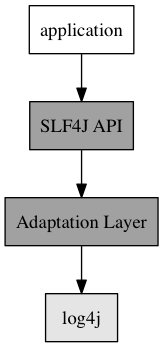
\includegraphics{slf4j.png}
\caption{SLF4j Using log4j}
\label{fig:slf4jlog4j}
\end{figure}

In figure \ref{fig:slf4jlog4j} the application uses SLF4J to log. It has been bound to use log4j libraries through the adaptation layer.

\subsubsection{Logging Without Configuration}

First we need to add the library to our project, as shown in the previous section.

To use the logger, we do the following:

\begin{lstlisting}[language=Java]
// imports
import java.util.logging.ConsoleHandler;
import java.util.logging.Level;
import java.util.logging.Logger;


// ...

System.setProperty(org.slf4j.impl.SimpleLogger.DEFAULT_LOG_LEVEL_KEY, "TRACE");
Logger logger = LoggerFactory.getLogger(this.getClass());
\end{lstlisting}
We import the needed classses. Log level can be one of trace, debug, info, warn, error, or off. trace is the lowest level and error is the highest. For example, warn level will log warn and error level messages. The default level is info \cite{simplelogger}. In our example we chose trace.

We can now write log messages:

\begin{lstlisting}[language=Java]
logger.error("Logging ERROR");
logger.warn("Logging WARN");
logger.info("Logging INFO");
logger.debug("Logging DEBUG");
\end{lstlisting}

With the SimpleLogger, our output will be:


handler.setLevel(Level.SEVERE);


\begin{lstlisting}
Dec 20, 2016 3:10:43 PM org.familysearch.viitanenm.DirectLoggingExample doIt
SEVERE: LOG LEVEL SEVERE
Dec 20, 2016 3:10:43 PM org.familysearch.viitanenm.DirectLoggingExample doIt
SEVERE: Logging ERROR
Dec 20, 2016 3:10:43 PM org.familysearch.viitanenm.DirectLoggingExample doIt
\end{lstlisting}

\begin{lstlisting}
Dec 20, 2016 3:10:43 PM org.familysearch.viitanenm.DirectLoggingExample doIt
SEVERE: Logging ERROR
Dec 20, 2016 3:10:43 PM org.familysearch.viitanenm.DirectLoggingExample doIt
WARNING: Logging WARN
Dec 20, 2016 3:10:43 PM org.familysearch.viitanenm.DirectLoggingExample doIt
INFO: Logging INFO
Dec 20, 2016 3:10:43 PM org.familysearch.viitanenm.DirectLoggingExample doIt
\end{lstlisting}

\begin{lstlisting}
Dec 20, 2016 3:10:43 PM org.familysearch.viitanenm.DirectLoggingExample doIt
FINEST: LOG LEVEL FINEST
Dec 20, 2016 3:10:43 PM org.familysearch.viitanenm.DirectLoggingExample doIt
SEVERE: Logging ERROR
Dec 20, 2016 3:10:43 PM org.familysearch.viitanenm.DirectLoggingExample doIt
WARNING: Logging WARN
Dec 20, 2016 3:10:43 PM org.familysearch.viitanenm.DirectLoggingExample doIt
INFO: Logging INFO
Dec 20, 2016 3:10:43 PM org.familysearch.viitanenm.DirectLoggingExample doIt
FINEST: Logging DEBUG
\end{lstlisting}